\documentclass[a4paper,12pt]{report}

\usepackage{graphicx} % For including images
\usepackage{geometry} % For margin customization
\geometry{
    left=1.5in,
    right=1in,
    top=1in,
    bottom=1in
}

\begin{document}

% Cover Page
\begin{titlepage}
    \centering
    {\LARGE ST. PAUL’S UNIVERSITY \par}
    \vspace{0.5cm}
    
    % School logo
    
\includegraphics[width=0.3\textwidth]{../img/logo.png} % Replace 'school-image-logo.png' with your actual logo file name
    
    \vspace{0.5cm}
    {\LARGE School of Communication and Computer Studies \par}
    \vspace{1.5cm}
    
    % Project Title
    {\Huge \textbf{FUNERAL MANAGEMENT SYSTEM IMPLEMENTATION} \par}
    \vspace{2cm}
    
    % Author Information
    {\Large \textbf{BY} \par}
    \vspace{0.5cm}
    {\Large TOM OUKO OKUDO \par}
    {\Large BSCNRB480122 \par}
    \vspace{2cm}
    
    % Department
    {\LARGE Department of Computer Science \par}
    \vfill
    
    % Submission Information
    {\large A research project submitted in partial fulfilment for the requirement of the award of a bachelor’s degree in computer science, Department of Computer Science, St. Paul’s University. \par}
    \vspace{1.5cm}
    
    % Date
    {\large November 2024 \par}
\end{titlepage}

% Declaration page
\newpage
% \chapter*{Declaration}
\addcontentsline{toc}{chapter}{Declaration} % Adds to Table of Contents

\begin{center}
    {\LARGE \textbf{DECLARATION}}
\end{center}

\vspace{1cm}

I do hereby declare without any reasonable doubt that the work presented is my own original and independent work and it has not been presented before to the Faculty of Science for the award of Bachelor of Science in Computer Science at ST. Paul’s University. No part of this report shall therefore be duplicated without my prior consent.

\vspace{2cm}

\begin{flushleft}
    \textbf{Name:} \underline{\hspace{4cm}} 
    \textbf{Reg No:} \underline{\hspace{4cm}} \\
    \vspace{0.5cm}
    \textbf{Signature:} \underline{\hspace{4cm}} \hspace{1cm} \textbf{Date:} \underline{\hspace{4cm}} \\
\end{flushleft}

\vspace{2cm}

\begin{flushleft}
    \textbf{Supervisor} \\

    \textbf{Name: MR. SAMUEL KARUGA} \\
    HOD Computer Science Department, St Paul’s University.
    
    \vspace{0.5cm}
    \textbf{Signature:} \underline{\hspace{4cm}}
\end{flushleft}

\vfill
\newpage

% Abstract page
\newpage
% \chapter*{Abstract}
\addcontentsline{toc}{chapter}{Abstract} % Adds to Table of Contents

\begin{center}
    {\LARGE \textbf{ABSTRACT}}
\end{center}

\vspace{1cm}

The funeral management system plays a crucial role in the funeral industry by streamlining operations, enhancing customer service, and ensuring efficient management of funeral services. This abstract delves into the key aspects of funeral management systems based on the provided sources.

Funeral management systems offer a comprehensive solution for funeral homes to manage various aspects of their operations efficiently. These systems provide features such as scheduling, inventory management, record-keeping, billing, invoicing, customer relationship management, and funeral planning tools. By utilizing advanced reporting features and customer relationship management, funeral homes can streamline their business services and sales effectively.

The primary objective of an FMS is to facilitate efficient management of funeral arrangements, from initial client contact to post-service follow-ups. Features typically include comprehensive client information management, automated documentation generation (such as contracts and permits), inventory tracking (including caskets, urns, and flowers), scheduling and coordination of services, and accounting integration for streamlined financial management.

The Funeral Management System is an indispensable tool for modern funeral homes seeking to enhance service delivery, optimize internal processes, and adapt to evolving industry demands. Its implementation represents a strategic investment towards achieving operational excellence, regulatory compliance, and sustained growth within the funeral service sector. Future research and development in FMS technology promise further innovations to meet the dynamic needs of funeral directors and their clientele.

\vfill
\newpage

\newpage
\chapter{Introduction}

\section{Background to the Study}
This project is aimed at developing a Funeral Management System (FMS), a tool designed to assist families and individuals in managing funeral arrangements during a difficult time. The FMS can be accessed by all users, allowing families to collaboratively plan arrangements either with funeral directors or independently from the comfort of their home. By providing a centralized platform, the system enables owners and managers to schedule services, communicate with clients, and manage various aspects of funeral arrangements more efficiently.

\section{Problem Statement}
The traditional, manual methods of handling funeral arrangements often lead to inefficiencies, disorganization, and additional stress for grieving families. As living standards improve, traditional funeral services struggle to meet evolving expectations for personalized, respectful, and well-organized experiences. To modernize the industry, funeral services require tools that streamline operations, integrate advanced information management technology, and provide culturally sensitive and humanized services. This FMS aims to reform traditional processes by incorporating these advanced functionalities and aligning with the contemporary demand for multi-level, personalized funeral service options.

\section{Objectives}
This project seeks to address the challenges associated with traditional funeral management methods by developing an efficient, accessible, and user-friendly funeral management system. The specific objectives include:
\begin{enumerate}
    \item To develop a website where customers can view products, services, and payment information.
    \item To make funeral services accessible to customers in distant locations.
    \item To enhance operational efficiency and service quality with features such as advanced reporting, calendar planning, and workload estimation.
    \item To automate funeral management tasks, reducing manual processes and increasing efficiency.
    \item To ease the workload on funeral service providers, reducing burnout by streamlining management processes.
    \item To improve customer satisfaction by providing a seamless online experience.
    \item To support timely, sensitive communication with clients through tools like email, SMS, and online portals, fostering trust and rapport.
    \item To improve financial management through features like budgeting, expense tracking, and financial reporting.
\end{enumerate}

\section{Project Schedule}
The following table outlines the time allocation for each project phase:

\begin{table}[h!]
    \centering
    \begin{tabular}{|c|l|c|}
        \hline
        \textbf{Phase} & \textbf{Task} & \textbf{Duration (Weeks)} \\
        \hline
        A & Data Collection & 3 \\
        B & Data Analysis & 2 \\
        C & Design Specification & 1 \\
        D & System/Database Design & 2 \\
        E & Coding & 3 \\
        F & Documentation & 3 \\
        \hline
    \end{tabular}
    \caption{Project Schedule}
    \label{table:schedule}
\end{table}

\section{Budget}
The following tables present the estimated budget required for project completion.

\subsection*{Materials}
\begin{table}[h!]
    \centering
    \begin{tabular}{|l|c|c|c|}
        \hline
        \textbf{Item} & \textbf{Quantity} & \textbf{Unit Cost (Ksh)} & \textbf{Total (Ksh)} \\
        \hline
        Transparent Paper & 1 Rim & 700 & 700 \\
        Embossed Paper & 1 Rim & 600 & 600 \\
        Ruler & 3 & 50 & 150 \\
        Photocopy Paper & 3 Rims & 500 & 1500 \\
        Biro Pens & 3 & 50 & 100 \\
        Flash Disk & 1 & 1200 & 1200 \\
        \hline
        \textbf{Total} & & & \textbf{4250} \\
        \hline
    \end{tabular}
    \caption{Material Costs}
    \label{table:material_costs}
\end{table}

\subsection*{Other Expenses}
\begin{table}[h!]
    \centering
    \begin{tabular}{|l|c|}
        \hline
        \textbf{Item} & \textbf{Amount (Ksh)} \\
        \hline
        Laptop & 80,000 \\
        Traveling & 3,000 \\
        Printing \& Typing & 3,000 \\
        Lunch & 5,000 \\
        Miscellaneous & 3,000 \\
        \hline
        \textbf{Total} & \textbf{94,000} \\
        \hline
    \end{tabular}
    \caption{Additional Expenses}
    \label{table:other_expenses}
\end{table}

\noindent \textbf{Grand Total:} Ksh 98,250

\section{Risks of the Funeral Management System}
Implementing the FMS presents various risks, including:

\begin{itemize}
    \item \textbf{Data Security and Privacy Concerns}: Sensitive personal and financial information is stored in the FMS, posing risks of data breaches, unauthorized access, and potential legal repercussions.
    \item \textbf{System Downtime and Technical Issues}: Dependence on technology introduces risks of technical failure or downtime, impacting service availability and customer satisfaction.
    \item \textbf{Training and Adoption Challenges}: Successful implementation requires adequate staff training. Resistance to change or inadequate training may limit system utilization.
    \item \textbf{Integration with Existing Systems}: Existing systems may be challenging to integrate with the FMS, requiring customization and troubleshooting.
    \item \textbf{Regulatory Compliance}: The FMS must meet legal and regulatory standards for record-keeping, consumer protection, and health and safety.
    \item \textbf{Customer Service and Communication}: Overreliance on automation may reduce personalization, impacting client satisfaction and reputation.
    \item \textbf{Cost Overruns and Budget Constraints}: Initial investments may lead to budgetary challenges if unforeseen expenses arise.
    \item \textbf{Vendor Dependency}: Dependence on external vendors poses risks related to vendor stability and responsiveness.
    \item \textbf{Scalability and Flexibility}: As funeral homes expand, the FMS must adapt to changing needs and additional functionalities.
    \item \textbf{Cultural Sensitivity and Ethical Considerations}: The system must respect diverse customs, religious practices, and cultural preferences to avoid misunderstandings or negative perceptions.
\end{itemize}

\newpage
\chapter{Literature Review}

\section{Introduction}
This chapter reviews the existing literature related to funeral management systems, providing context for the development of this project. The literature highlights both the advancements and challenges in funeral management, addressing how existing systems manage processes such as scheduling, payment handling, and inventory management. An understanding of these systems will provide a foundation for proposing improvements through this project.

The literature also evaluates various aspects of funeral management, including the integration of technology in a traditionally manual industry. This review will explore related systems, identify their limitations, and demonstrate how the proposed Funeral Management System (FMS) aims to address these shortcomings by offering a more efficient and user-friendly platform.

\section{Related Systems}
Several funeral management systems have been developed and deployed in recent years, aiming to improve the efficiency of funeral planning and management. This section discusses some of the key systems that have been developed to manage funeral services, providing insight into their features and operations.

\subsection{System 1: Funeral Home Management Software (FHMS)}
Funeral Home Management Software (FHMS) is a comprehensive solution designed for funeral homes to streamline their operations. It integrates features such as client management, inventory tracking, scheduling, and invoicing. This system helps funeral service providers manage their day-to-day tasks, including funeral arrangements, customer records, and financial transactions.

FHMS provides an intuitive interface for funeral directors and clients alike, enabling easy access to service details, inventory, and billing. The system also supports financial management, allowing users to track payments and generate reports. However, FHMS primarily focuses on service providers rather than clients, and the lack of an online client portal for families seeking funeral services limits its accessibility.

\subsection{System 2: The Death Care Manager (DCM)}
The Death Care Manager (DCM) is an online platform designed to manage end-of-life services. It offers features such as funeral planning, obituary creation, and family collaboration tools. DCM focuses on assisting families through the grieving process by allowing them to coordinate with funeral homes, share information, and personalize funeral arrangements online. 

The system allows clients to access their funeral planning tools from any location, offering flexibility in managing funeral arrangements. However, it lacks integration with local funeral service providers, making it difficult for users to seamlessly connect with funeral homes. Additionally, it does not support real-time tracking of funeral service progress, which could lead to miscommunications and scheduling issues.

\subsection{System 3: Funeral Planning Tool (FPT)}
Funeral Planning Tool (FPT) is an online solution designed to assist families with funeral planning. This platform offers resources for planning a funeral, including casket and urn selection, service options, and funeral expenses tracking. Families can create funeral plans, invite loved ones to contribute, and share details of the service arrangements with other family members.

FPT is user-friendly and allows families to manage all aspects of funeral planning from a single interface. However, one of the key limitations of FPT is the lack of a centralized communication system between funeral service providers and families. This gap can cause delays in confirming service details, such as transport and inventory availability. The system’s payment system is also not integrated with external payment gateways, which could be a problem for users in different regions.

\section{Limitations of Existing Systems}
While funeral management systems like FHMS, DCM, and FPT offer some benefits in streamlining operations, they are not without limitations. Below are the key weaknesses of these systems:

\subsection{Lack of Client-Centered Features}
Most of the current funeral management systems, such as FHMS, are designed with service providers in mind. While they focus on improving the internal operations of funeral homes, they do not provide adequate tools for families and clients to manage the funeral planning process. For instance, families often cannot directly access funeral services, track service progress, or collaborate with funeral directors in real-time.

\subsection{Limited Online Accessibility}
Although systems like DCM and FPT provide some online tools, they still suffer from limited accessibility features. Users often face difficulties in accessing funeral services from distant locations or across regions. The lack of mobile compatibility and user-friendly client portals in many systems prevents families from managing arrangements efficiently, especially in times of grief.

\subsection{Inadequate Integration with Service Providers}
Another common limitation in existing systems is poor integration with funeral service providers. Systems like DCM and FPT do not provide a seamless connection between families and funeral homes. Without integration, users are forced to manually contact funeral homes to finalize service arrangements. Furthermore, there is often no real-time communication to track the progress of service delivery, leading to potential scheduling conflicts and delays.

\subsection{Financial Management Challenges}
Most existing systems do not offer robust financial management features. While FHMS includes invoicing and payment tracking, systems like DCM and FPT lack integrated payment gateways, which complicates the payment process. Users also face challenges in tracking funeral expenses in detail, including the cost of services, transport, and inventory.

\section{How the Proposed Solution Will Handle These Weaknesses}
The proposed Funeral Management System (FMS) aims to address the limitations of existing systems by incorporating the following features:

\subsection{Client-Centered Design}
Unlike existing systems that focus primarily on service providers, the FMS will be designed to put families and clients at the center. The system will offer a user-friendly interface that allows families to manage funeral plans, collaborate with funeral homes, and track progress in real-time. Clients will have access to all service details, from casket selection to funeral logistics, in one platform, ensuring transparency and peace of mind.

\subsection{Enhanced Online Accessibility and Mobile Support}
The FMS will be fully accessible online and optimized for both desktop and mobile devices. This will enable families to access the platform from anywhere, at any time, and manage their arrangements without the need to visit a funeral home physically. The mobile-friendly design will ensure ease of use, even during stressful times.

\subsection{Seamless Integration with Service Providers}
To address the issue of integration with funeral service providers, the FMS will feature a system that connects families directly with funeral homes and other service providers. By providing real-time updates on service availability, scheduling, and inventory, families will be able to manage the entire funeral process without delays or miscommunications. This integration will enhance the efficiency of service delivery and improve the overall customer experience.

\subsection{Comprehensive Financial Management Tools}
The FMS will offer integrated financial management tools that allow users to track all funeral-related expenses in real-time. Users will be able to view and manage their budget, make payments through secure payment gateways, and receive detailed financial reports. This will ensure that families can manage the financial aspects of the funeral process with transparency and control.

\section{Conclusion}
This chapter has reviewed related systems in funeral management and highlighted their strengths and weaknesses. While existing systems have made significant progress in improving funeral services, they still fall short in terms of client-centered features, accessibility, integration with service providers, and financial management. The proposed Funeral Management System will address these shortcomings by offering a more comprehensive, integrated, and user-friendly platform for both funeral service providers and clients.

\newpage
\chapter{Methodology}

\section{Introduction}
This chapter outlines the methodology for developing the Funeral Management System (FMS). It describes how the project will be carried out, the tools and technologies to be used, data collection and analysis methods, and the system requirements. A project schedule and budget are also provided to ensure the work progresses efficiently and within allocated resources.

\section{Project Design}
The design of the Funeral Management System will involve both frontend and backend development. This section outlines the development methodology, the architecture of the system, and the specific tools and technologies to be used.

\subsection{Development Methodology}
The Waterfall Development methodology will be employed for this project. Waterfall is a linear and sequential development process where each phase must be completed before proceeding to the next. This methodology is well-suited for projects with clearly defined requirements.

\subsubsection{Justification for Using Waterfall}
The Waterfall methodology was selected because:
\begin{itemize}
    \item The project has clear, well-defined requirements.
    \item It allows for systematic documentation and testing after each phase.
    \item It ensures that there is little scope for changes once the project moves into the development phase.
\end{itemize}

% \begin{figure}[ht]
% \centering
% \includegraphics[width=0.7\textwidth]{water-fall-img.png}
% \caption{Waterfall Development Methodology}
% \label{fig:waterfall_model}
% \end{figure}

The development process is broken down into distinct phases: Requirements, Design, Implementation, Testing, and Deployment. Each phase is completed before the next begins, ensuring a controlled and predictable flow of development.

\section{Design Procedures}
The system design follows a structured approach that focuses on both the frontend user interface and the backend logic for efficient service management.

\subsection{System Architecture}
The system architecture follows a client-server model where the frontend communicates with the backend through HTTP requests. The system will be built using a combination of web technologies to ensure a smooth user experience and efficient data management.

\subsubsection{Frontend Architecture}
The frontend architecture will be based on:
\begin{itemize}
    \item HTML5: To structure the content on web pages.
    \item CSS (Bootstrap): To style the system and provide a responsive, mobile-friendly design.
    \item JavaScript: For dynamic features and client-side validation.
\end{itemize}

\subsubsection{Backend Architecture}
The backend will be built with:
\begin{itemize}
    \item PHP: For server-side logic, including business logic and user management.
    \item MySQL: To handle data storage, including client records, service details, and financial transactions.
\end{itemize}

% \begin{figure}[ht]
% \centering
% \includegraphics[width=0.8\textwidth]{Client-Server-img.png}
% \caption{Client-Server Architecture of the System}
% \label{fig:client_server_architecture}
% \end{figure}

\subsection{User Interface Design}
The design of the user interface focuses on usability and responsiveness. The UI will be clean, easy to navigate, and accessible to all users, including funeral home staff and family members.

\begin{itemize}
    \item Responsive Design: The design will adapt to different screen sizes using Bootstrap's grid system.
    \item User-Centered Design: Navigation will be intuitive, with clearly labeled sections for scheduling, inventory, and payment management.
    \item Client-Side Validation: JavaScript will ensure proper form validation and error handling.
\end{itemize}

\section{System Requirements}
The following are the hardware and software requirements necessary for developing, deploying, and running the Funeral Management System.

\subsection{Hardware Requirements}
The following hardware resources are required for the development and deployment phases:
\begin{table}[ht]
\centering
\begin{tabular}{|c|c|}
\hline
\textbf{Component} & \textbf{Specification} \\
\hline
\textbf{Development Machine} & 8GB RAM, 2.5 GHz Processor \\
\textbf{Server} & Cloud Server or Local Server (with Apache) \\
\hline
\end{tabular}
\caption{Hardware Requirements for Development and Deployment}
\label{tab:hardware_requirements}
\end{table}

\subsection{Software Requirements}
The software requirements for this project are as follows:
\begin{table}[ht]
\centering
\begin{tabular}{|c|c|}
\hline
\textbf{Software} & \textbf{Version/Description} \\
\hline
\textbf{Operating System} & Windows, Linux, or macOS \\
\textbf{Frontend} & HTML5, CSS (Bootstrap), JavaScript \\
\textbf{Backend} & PHP 7.x or higher \\
\textbf{Database} & MySQL 5.x or higher \\
\textbf{Development Tools} & Visual Studio Code, XAMPP/WAMP \\
\textbf{Database Management} & phpMyAdmin \\
\hline
\end{tabular}
\caption{Software Requirements}
\label{tab:software_requirements}
\end{table}

\section{Data Collection and Analysis (Needs Assessment)}
To design a system that effectively addresses user needs, data will be collected from key stakeholders, including funeral directors, administrative staff, and clients. This section outlines the methods for gathering data and analyzing it to determine the system's features and functionalities.

\subsection{Data Collection Methods}
The following methods will be used for collecting data:
\begin{itemize}
    \item Surveys: A survey will be distributed to funeral directors and clients to collect feedback on existing systems and desired features.
    \item Interviews: In-depth interviews with key stakeholders will provide detailed insights into operational challenges.
    \item Observations: On-site visits will be conducted to observe the day-to-day operations of funeral homes.
\end{itemize}

\subsection{Data Analysis}
After collecting the data, it will be analyzed to:
\begin{itemize}
    \item Identify the most important features for the system (e.g., service scheduling, payment tracking).
    \item Assess the weaknesses of current systems to ensure that these issues are addressed in the new design.
    \item Prioritize features based on user feedback and their impact on the funeral home's operations.
\end{itemize}

% \begin{figure}[ht]
% \centering
% \includegraphics[width=0.7\textwidth]{data_analysis_process.png}
% \caption{Data Collection and Analysis Process}
% \label{fig:data_analysis_process}
% \end{figure}

\subsection{Tools for Data Analysis}
The following tools will be used for analyzing the collected data:
\begin{itemize}
    \item Microsoft Excel: To organize survey responses and perform basic statistical analysis.
    \item SPSS: For more advanced statistical analysis if necessary.
    \item NVivo: For qualitative analysis of interview data and open-ended survey responses.
\end{itemize}

\section{Project Schedule and Budget}
A detailed schedule and budget are essential to ensure the project progresses on time and within budget. The following sections outline the project timeline and estimated costs.

\subsection{Project Schedule}
The estimated project duration is 6 months. The project will be divided into the following phases:

\begin{table}[ht]
\centering
\begin{tabular}{|c|c|}
\hline
\textbf{Phase} & \textbf{Duration} \\
\hline
Requirements Gathering & 2 weeks \\
System Design & 3 weeks \\
Frontend and Backend Development & 8 weeks \\
Testing & 4 weeks \\
Deployment & 2 weeks \\
Final Review & 2 weeks \\
\hline
\end{tabular}
\caption{Project Schedule}
\label{tab:project_schedule}
\end{table}

\subsection{Project Budget}
The estimated budget for the project includes the following components:

\begin{table}[ht]
\centering
\begin{tabular}{|c|c|}
\hline
\textbf{Component} & \textbf{Cost} \\
\hline
Software Licenses & \$0 (open-source tools) \\
Server Hosting & \$100/month (cloud hosting) \\
Development Tools & \$0 (open-source IDEs) \\
Personnel Costs & \$0 (self-developed) \\
\hline
\end{tabular}
\caption{Estimated Project Budget}
\label{tab:project_budget}
\end{table}

Total estimated budget: \$ 600 for the entire project.

\section{Conclusion}
This chapter has outlined the methodology for the development of the Funeral Management System, focusing on project design, tools, system requirements, data collection and analysis methods, and the project schedule and budget. The approach includes a systematic development process using PHP, MySQL, HTML5, CSS (Bootstrap), and JavaScript to ensure the system is user-friendly, efficient, and meets the needs of the stakeholders.

\newpage
\chapter{System Analysis}

\section{Introduction}
This chapter provides a detailed analysis of the current system and the proposed improvements for the Funeral Management System (FMS). It aims to explore the existing workflows, identify inefficiencies, and outline the necessary system requirements that the new system will address. The analysis includes flowcharts, Data Flow Diagrams (DFDs), UML diagrams, and context diagrams to give a comprehensive understanding of the existing processes.

\section{Current System Analysis}
This section analyzes the current system, focusing on how funeral homes manage their services, including scheduling, inventory management, client information, financial tracking, and reporting.

\subsection{Flowcharts of Current System}
Flowcharts represent the logical flow of processes in the current system. Below is a basic flowchart for the funeral service management system’s existing process.

\begin{figure}[ht]
\centering
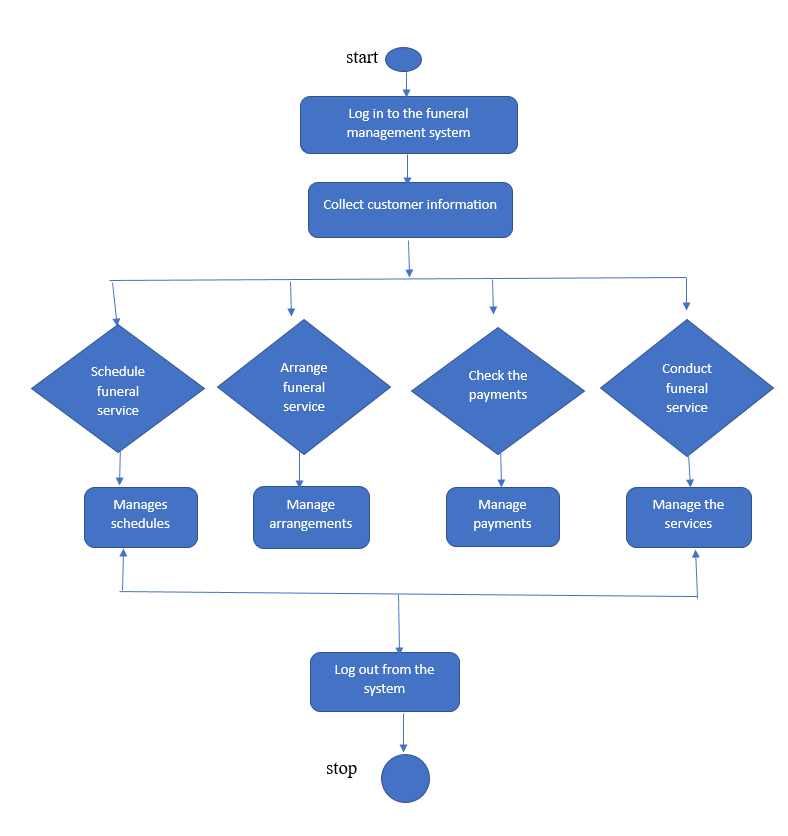
\includegraphics[width=0.7\textwidth]{../img/flow-chart.png}
\caption{Flowchart of Current System Process}
\label{fig:current_system_flowchart}
\end{figure}

\subsection{Data Flow Diagram (DFD) of Current System}
A Data Flow Diagram (DFD) helps visualize the flow of information within the current system. Below is a level-0 DFD showing the major processes and data flows in the existing system.

\begin{figure}[ht]
\centering
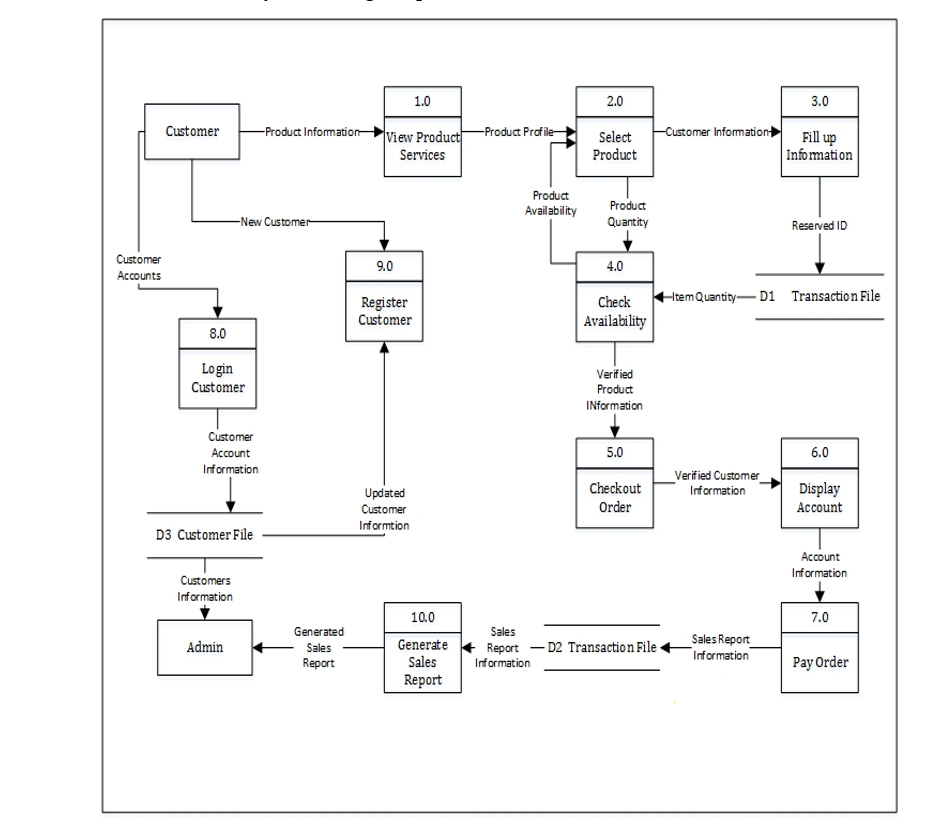
\includegraphics[width=0.8\textwidth]{../img/activity.png}
\caption{Level 0 DFD of Current System}
\label{fig:dfd_level_0}
\end{figure}

The DFD illustrates the interaction between the system’s external entities (e.g., clients, funeral directors, payment systems) and its internal processes (e.g., scheduling, inventory, billing).

\subsection{Context Diagram of Current System}
A Context Diagram provides a high-level view of the entire system, showing how it interacts with external entities. 
Below is the context diagram for the current system, which gives an overview of the external entities and their interactions with the system.

% \begin{figure}[ht]
% \centering
% \includegraphics[width=0.7\textwidth]{current_system_context.png}
% \caption{Context Diagram of Current System}
% \label{fig:current_system_context}
% \end{figure}

\subsection{UML Diagram of Current System}
A Unified Modeling Language (UML) diagram can represent the current system’s class structure and interactions. The following diagram represents the basic structure of the system, including key entities such as `Client`, `FuneralService`, `Inventory`, and `Payment`.

\begin{figure}[ht]
\centering
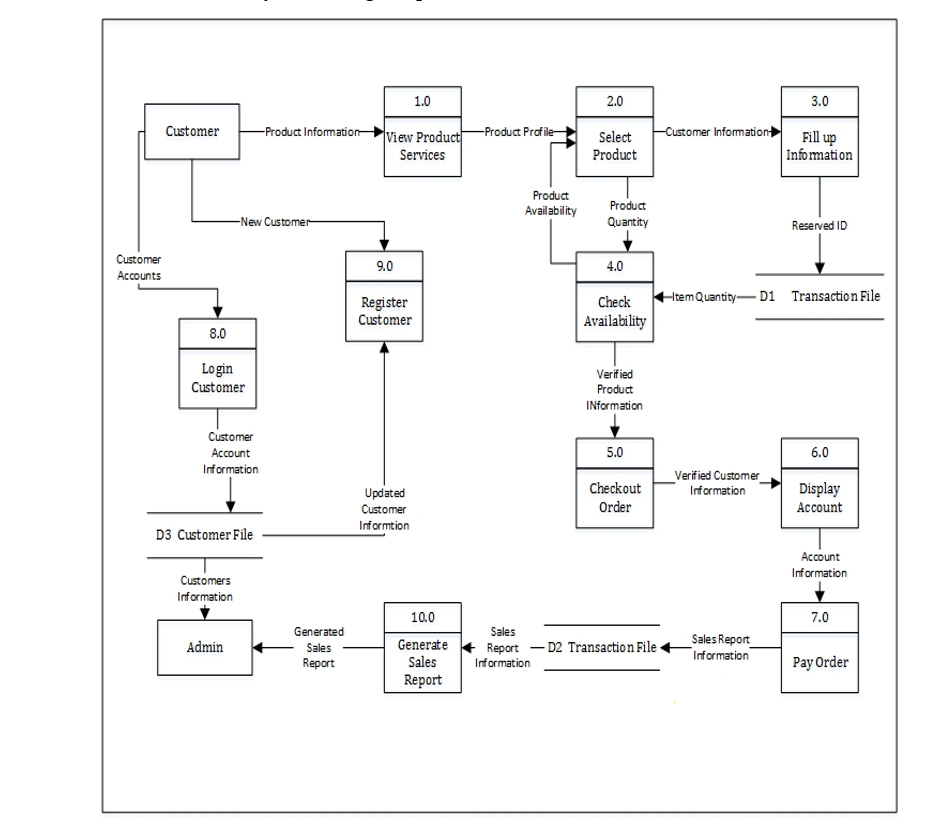
\includegraphics[width=0.8\textwidth]{../img/activity.png}
\caption{UML Diagram of Current System}
\label{fig:current_system_uml}
\end{figure}

The UML diagram highlights the relationships between different system components, providing a visual representation of the data entities and their interactions.

\section{System Requirements}
This section outlines the system requirements that are critical for the development of the Funeral Management System. These requirements are divided into **functional** and **non-functional** categories.

\subsection{Functional Requirements}
Functional requirements define the core functions that the system must perform. These are features that will help automate and streamline the processes in the funeral home.

\begin{itemize}
    \item User Authentication and Authorization: The system must allow users (funeral directors, staff, clients) to create accounts, log in securely, and have role-based access control.
    \item Service Booking: The system should enable scheduling funeral services, including setting dates, times, and locations, as well as tracking service progress.
    \item Inventory Management: The system must manage inventory such as coffins, caskets, urns, and other essential items, allowing funeral homes to update stock levels in real-time.
    \item Client Information Management: The system must store client details, including personal information, services requested, and payment history.
    \item Payment Management: The system should track payments, issue invoices and receipts, and calculate service costs including taxes and discounts.
    \item Reporting: The system must generate reports on services, inventory, payments, and financial summaries for management review.
\end{itemize}

\subsection{Non-Functional Requirements}
Non-functional requirements define the system’s operational qualities, such as performance, usability, and security.

\begin{itemize}
    \item Performance: The system must be responsive, with pages loading in less than 3 seconds.
    \item Scalability: The system must handle increased numbers of users and transactions as the funeral home grows.
    \item Security: The system should implement encryption for sensitive data (e.g., passwords, payment details) and ensure secure communication (SSL/TLS).
    \item Usability: The system must be user-friendly, with an intuitive interface that staff with minimal technical knowledge can use efficiently.
    \item Availability: The system must be available 24/7, with backup and recovery mechanisms in place in case of failure.
    \item Compliance: The system must comply with relevant local regulations regarding data privacy, financial transactions, and record-keeping.
\end{itemize}

\section{Conclusion}
This chapter provided a detailed analysis of the current system used in managing funeral services and highlighted the inefficiencies that the proposed system aims to address. By incorporating flowcharts, DFDs, context diagrams, and UML diagrams, the current system's structure and workflows were examined. The system requirements, both functional and non-functional, were then outlined to ensure the proposed system will meet the needs of the funeral home while improving efficiency, security, and overall service delivery.

\newpage
\chapter{System Design}

\section{Introduction}
This chapter provides a detailed description of the system design for the Funeral Management System (FMS). It covers the architectural design, database design, and user interface design. The system's design will ensure that all components function seamlessly, aligning with the functional and non-functional requirements outlined earlier. Tools such as Entity Relationship Diagrams (ERDs), Data Flow Diagrams (DFDs), and UML diagrams are used for a comprehensive design representation.

\section{Architectural Design}
The architectural design of the system follows a three-tier architecture which is divided into three primary layers:

\begin{itemize}
    \item \textbf{Presentation Layer (Frontend)}: This layer is responsible for the user interface, which is built using HTML, CSS (Bootstrap), and JavaScript.
    \item \textbf{Application Layer (Backend)}: This layer processes the business logic and data handling, built using PHP and MySQL for database interaction and management.
    \item \textbf{Data Layer (Database)}: The database stores the system’s data such as client information, funeral services, payments, and inventory. MySQL is used as the database management system.
\end{itemize}

The system uses a client-server architecture, where the frontend interacts with the backend via HTTP requests. The backend handles the logic and communicates with the database to return the necessary responses to the frontend.

\subsection{System Architecture Diagram}
Below is the architectural design of the system, showing the interaction between the client-side (frontend), server-side (backend), and database.

\begin{figure}[ht]
\centering
\begin{minipage}{0.45\textwidth}
    \centering
    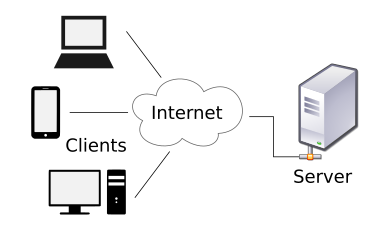
\includegraphics[width=\linewidth]{../img/Client-Server.png}
    \caption{System Architecture Overview}
    \label{fig:system_architecture_1}
\end{minipage}%
\hfill
\begin{minipage}{0.45\textwidth}
    \centering
    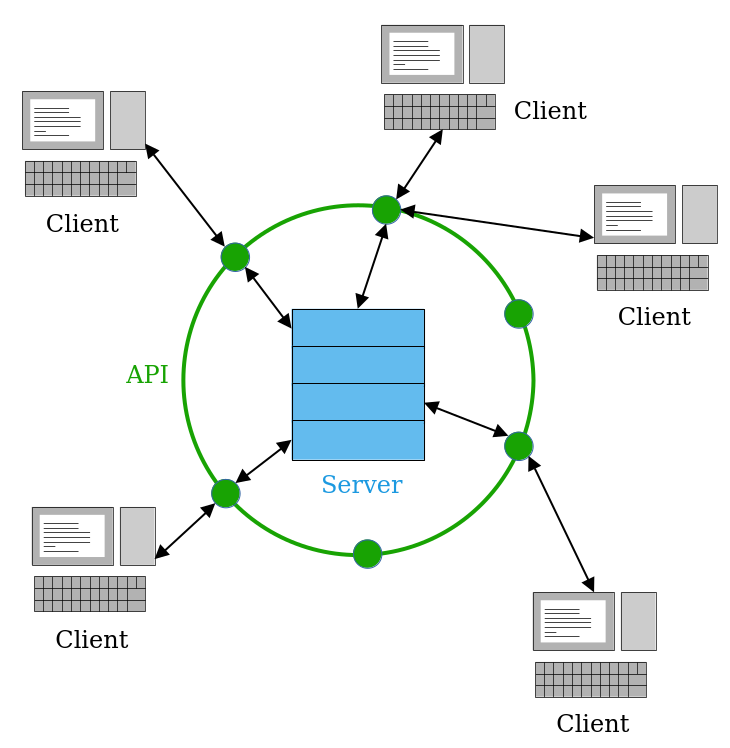
\includegraphics[width=\linewidth]{../img/cli-server.png}
    \caption{Client-Server Interaction}
    \label{fig:system_architecture_2}
\end{minipage}
\end{figure}

\section{Database Design}
In this section, we provide a detailed design of the database using an Entity Relationship Diagram (ERD). The ERD outlines the relationship between key entities in the system, such as `Clients`, `Funeral Services`, `Payments`, and `Inventory`.

\subsection{Entity Relationship Diagram (ERD)}
The following diagram shows the relationships between the primary entities in the system:

\begin{figure}[ht]
\centering
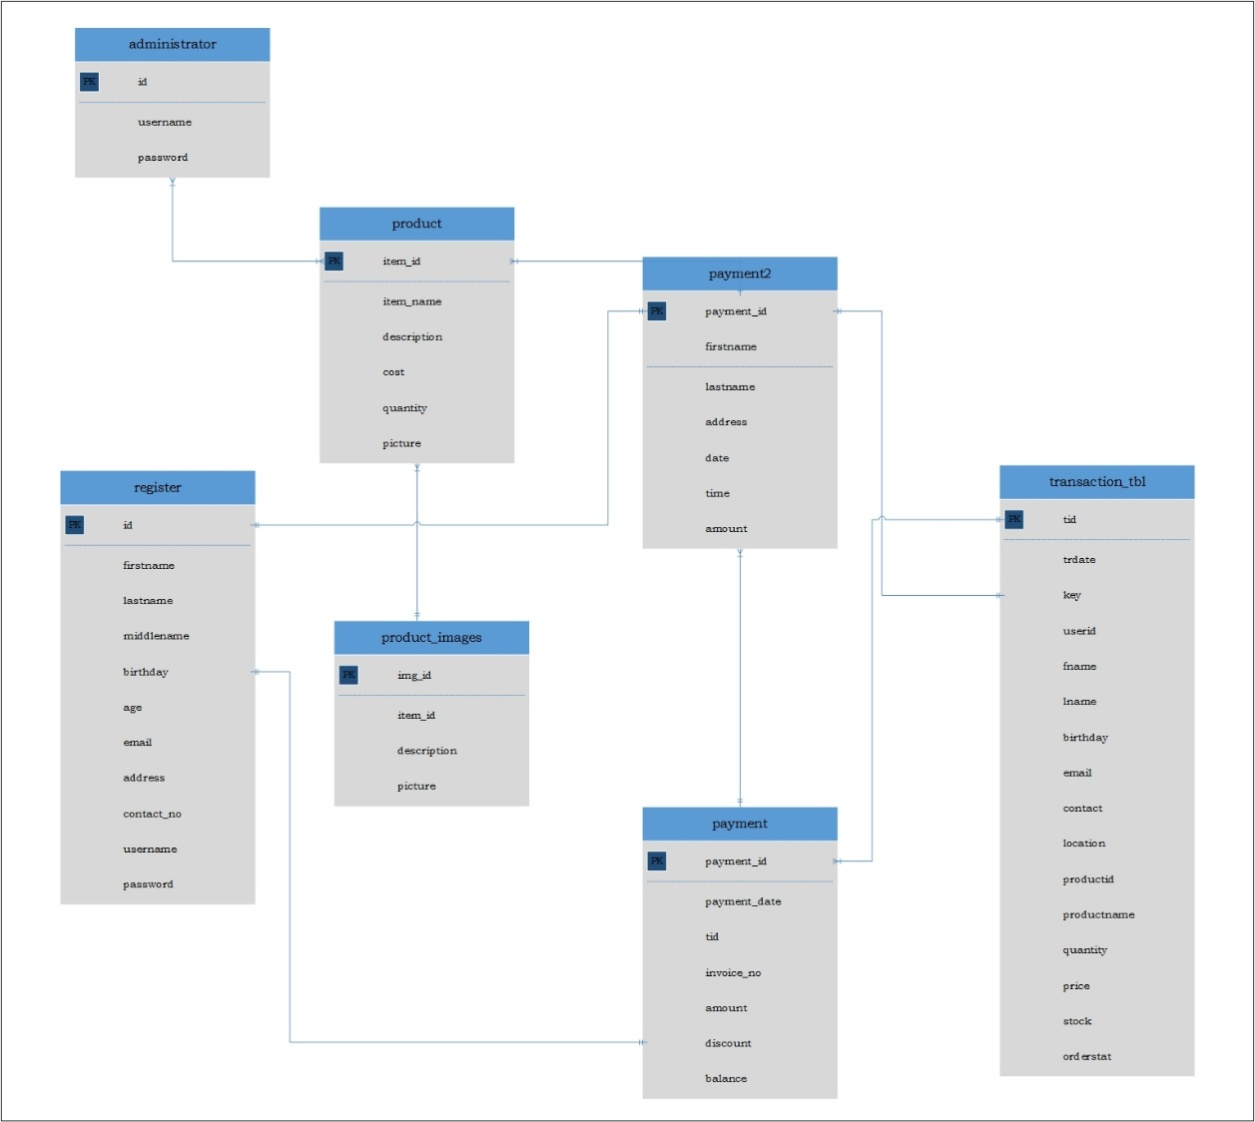
\includegraphics[width=0.8\textwidth]{../img/erd.png}
\caption{Entity Relationship Diagram (ERD)}
\label{fig:erd}
\end{figure}

\subsection{Database Schema}
The database schema describes how the data is stored in the system. Below is an example of the table schema for the `Clients` table:

\begin{table}[ht]
\centering
\begin{tabular}{|l|l|l|}
\hline
\textbf{Column Name} & \textbf{Data Type} & \textbf{Description} \\ \hline
client\_id & INT & Primary Key, Auto Increment \\ \hline
first\_name & VARCHAR(100) & Client’s First Name \\ \hline
last\_name & VARCHAR(100) & Client’s Last Name \\ \hline
contact\_number & VARCHAR(15) & Client’s Contact Number \\ \hline
email & VARCHAR(100) & Client’s Email Address \\ \hline
address & TEXT & Client’s Address \\ \hline
\end{tabular}
\caption{Clients Table Schema}
\label{tab:clients_schema}
\end{table}

This schema will be applied to all entities in the system to ensure consistency and proper data management.

\section{User Interface Design}
The user interface (UI) of the Funeral Management System is designed to be intuitive and easy to use. It incorporates responsive design principles to ensure that the system is usable on both desktop and mobile devices. The UI is built using HTML, CSS (Bootstrap), and JavaScript, with a focus on simplicity and functionality.

\subsection{UI Components}
The system contains several key UI components:

\begin{itemize}
    \item \textbf{Login Page}: A secure login page for both staff and clients, featuring username and password fields.
    \item \textbf{Dashboard}: Displays key information such as upcoming services, inventory status, and payment history.
    \item \textbf{Service Booking Form}: Allows clients to book funeral services and select service preferences.
    \item \textbf{Inventory Management}: Displays inventory data and enables funeral home staff to manage inventory items.
    \item \textbf{Client Management}: A page that allows staff to view and manage client details and service history.
    \item \textbf{Payment Page}: Enables tracking of client payments and the issuance of invoices.
\end{itemize}

\subsection{Responsive Design with Bootstrap}
Bootstrap ensures that the UI is responsive and adapts seamlessly to different screen sizes. The UI components adjust dynamically to fit the screen size, making the system accessible across a variety of devices, from desktop computers to mobile phones.

\subsection{User Interface Example}
Below is an example of the UI for the dashboard page. It displays an overview of the system’s current status, such as upcoming funeral services and inventory levels.

\begin{figure}[ht]
\centering
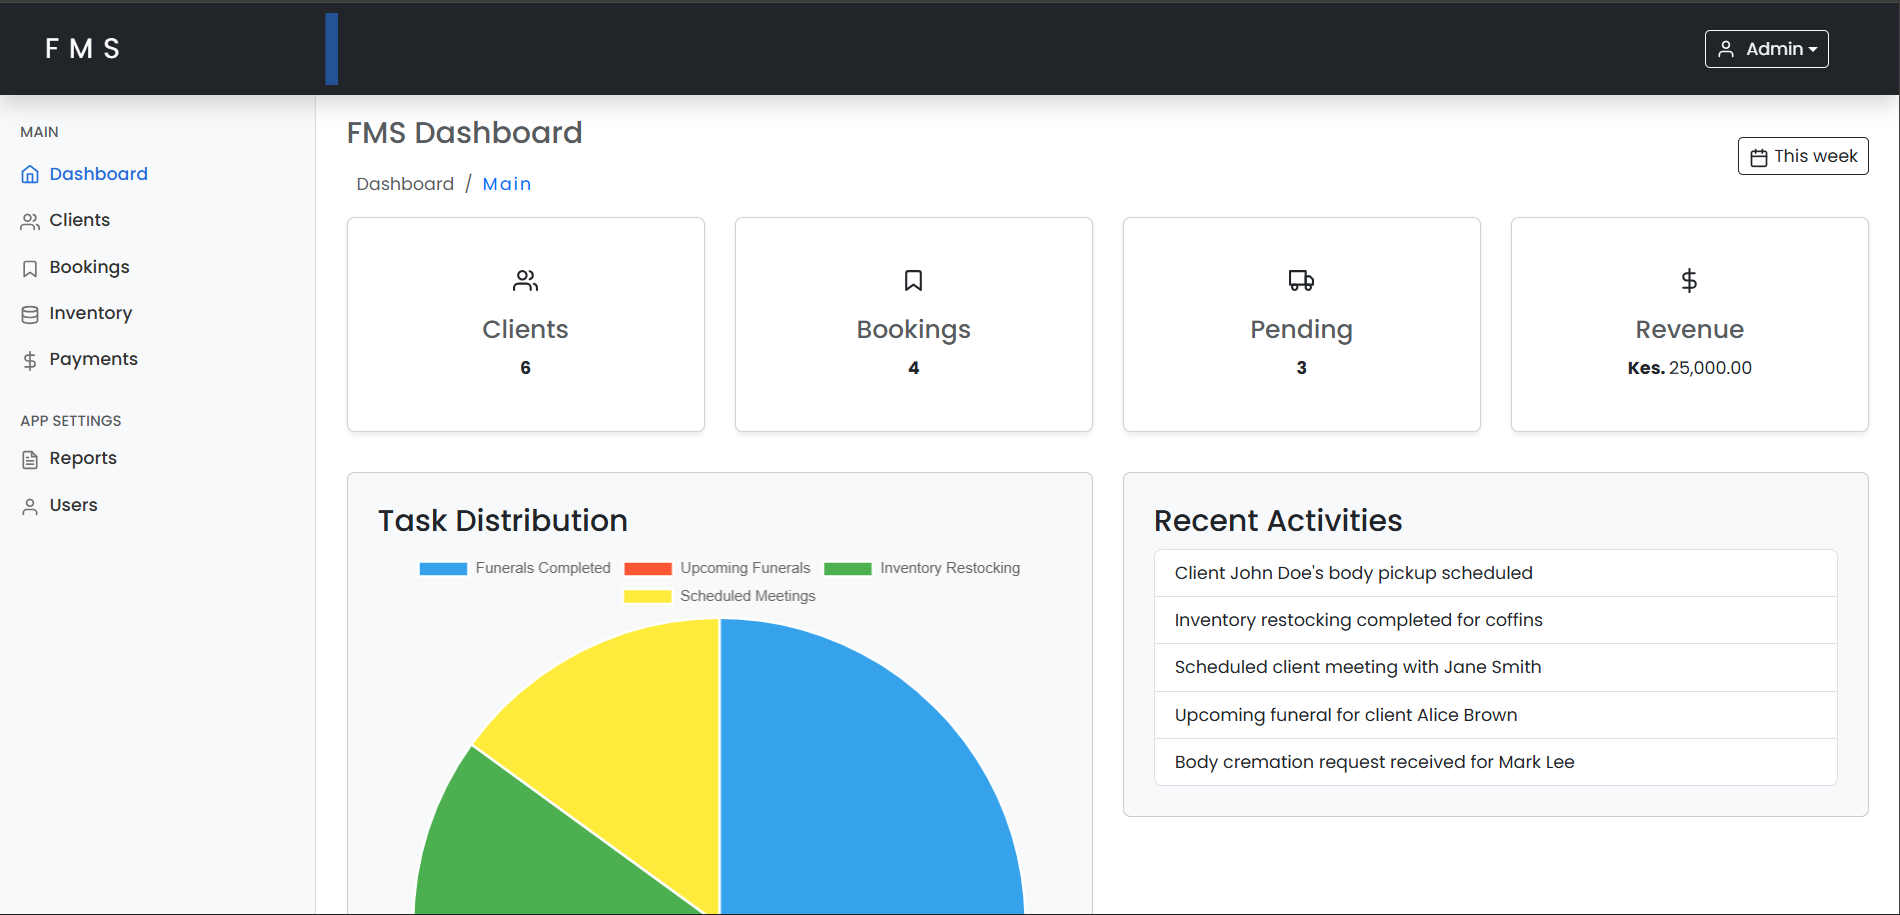
\includegraphics[width=0.8\textwidth]{../img/dashboard.png}
\caption{Dashboard User Interface}
\label{fig:dashboard_ui}
\end{figure}


% Reports
\begin{figure}[ht]
    \centering
    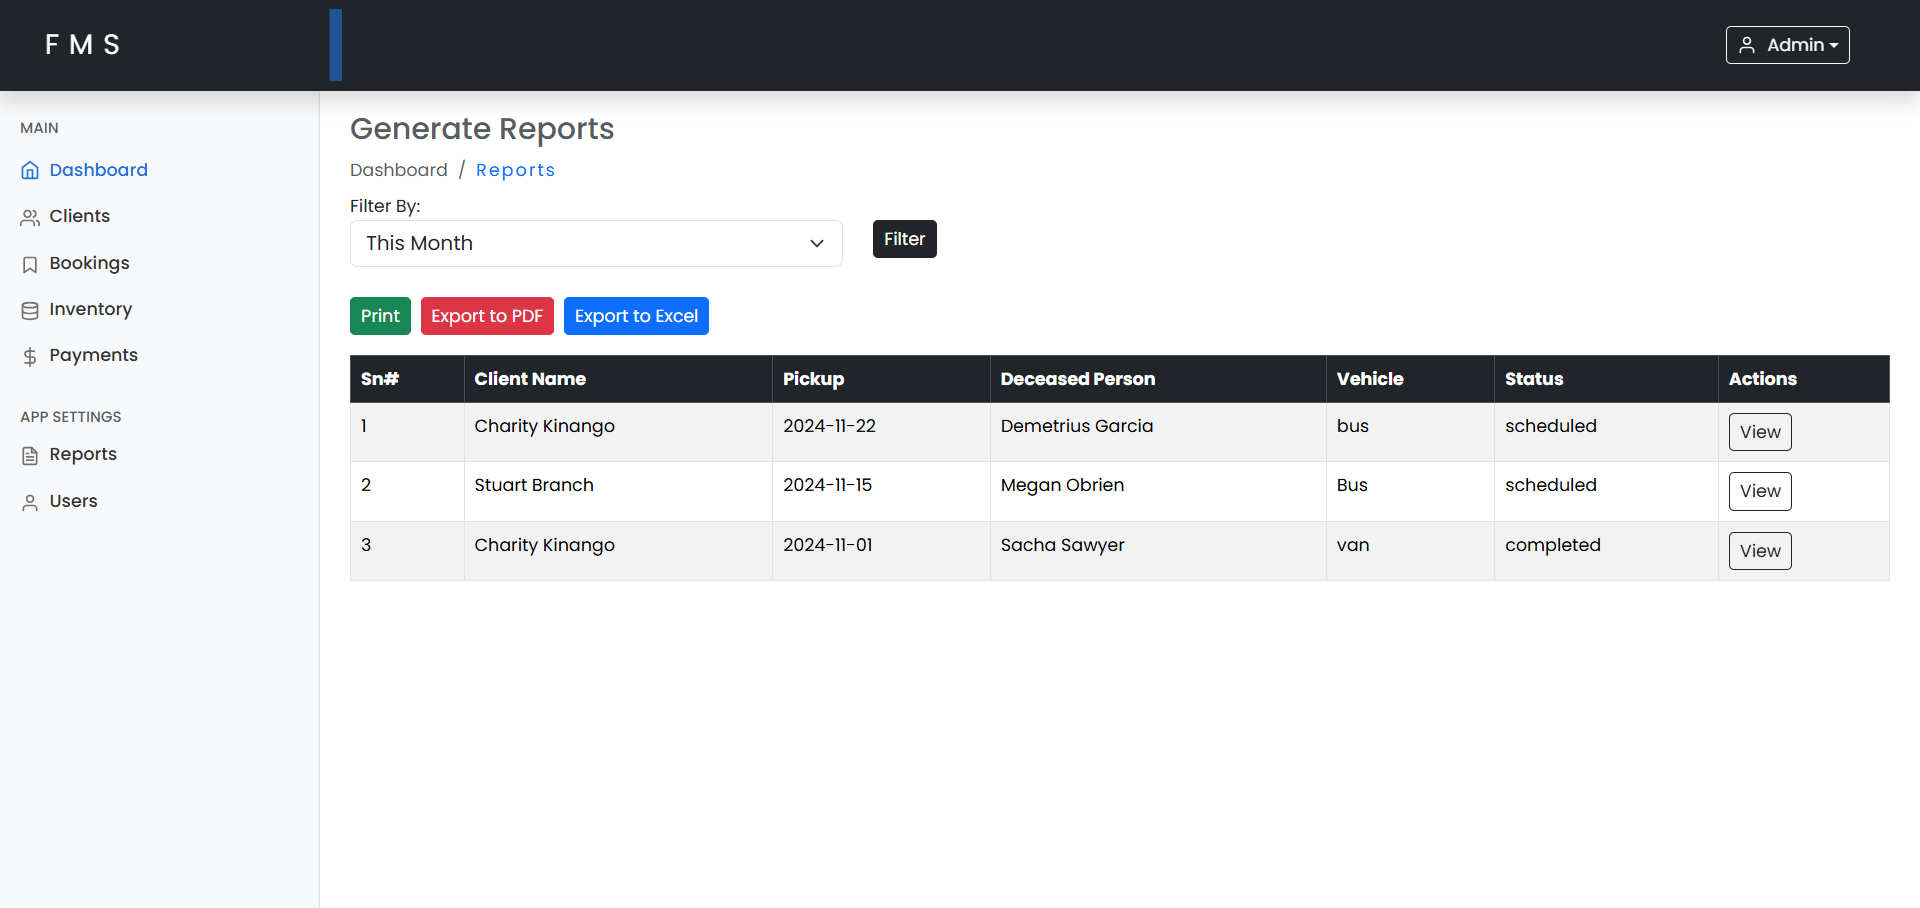
\includegraphics[width=0.8\textwidth]{../img/resports.png}
    \caption{Reports User Interface}
    \label{fig:reports_ui}
\end{figure}

% Login
\begin{figure}[ht]
    \centering
    
\includegraphics[width=0.8\textwidth]{../img/login.png}
    \caption{Login User Interface}
    \label{fig:login_ui}
\end{figure}

% UI
\subsection{User Experience (UX) Considerations}
The design emphasizes the following UX principles:
\begin{itemize}
    \item \textbf{Simplicity}: The interface is kept clean and user-friendly with easy navigation.
    \item \textbf{Consistency}: Design elements like colors, buttons, and typography are consistent across all pages.
    \item \textbf{Accessibility}: The system follows web accessibility guidelines (e.g., WCAG) to ensure it is usable by people with disabilities.
    \item \textbf{Feedback}: The system provides feedback for user actions, such as confirmation of bookings or payments.
\end{itemize}

\section{Conclusion}
This chapter presented the design of the Funeral Management System, covering architectural design, database design, and user interface design. The system architecture follows a three-tier model, with a client-server structure for seamless interaction between the frontend, backend, and database. The ERD and database schema ensure that data is structured and stored efficiently. The user interface is designed to be responsive and intuitive, ensuring a positive experience for both clients and staff. With this design blueprint, the system is ready for development and implementation.

\newpage
\chapter*{References}

\begin{enumerate}
    \item Software Advice. (n.d.). \textit{Funeral home software}. Retrieved from https://www.softwareadvice.com/funeral-home/
    
    \item Gather. (2020, November 4). \textit{Funeral management system: A guide for funeral homes}. Retrieved from https://gather.app/blog/funeral-management-system/
    
    \item Select Funerals. (n.d.). \textit{Select quality management system}. Retrieved from https://selectfunerals.com/79/Select-Quality-Management-System.html
    
    \item EY. (2020, December 1). \textit{The shift to intelligent facilities management}. Retrieved from https://www.ey.com/en_us/strategy-transactions/the-shift-to-intelligent-facilities-management
    
    \item GeeksforGeeks. (2022, July 15). \textit{Software development life cycle (SDLC)}. Retrieved from https://www.geeksforgeeks.org/software-development-life-cycle-sdlc/
    
    \item Miro. (n.d.). \textit{What is a UML diagram?}. Retrieved from https://miro.com/diagramming/what-is-a-uml-diagram/
    
    \item APM. (n.d.). \textit{What is project management?}. Retrieved from https://www.apm.org.uk/resources/what-is-project-management/
    
    \item AltexSoft. (2020, May 12). \textit{Functional and non-functional requirements: Specification and types}. Retrieved from https://www.altexsoft.com/blog/functional-and-non-functional-requirements-specification-and-types/
    
    \item InterviewBit. (2022, October 17). \textit{System architecture}. Retrieved from https://www.interviewbit.com/blog/system-architecture/
    
    \item Global Legal Post. (2021, January 19). \textit{Planning for system upgrades and future improvement phases}. Retrieved from https://www.globallegalpost.com/news/planning-for-system-upgrades-and-future-improvement-phases-1311896976
\end{enumerate}




















\end{document}
